%!TEX root = ../report.tex

% 
% Architecture
% 

\section{Architecture}
\label{sec:arch}

The problem addressed in this thesis is to design and implement an interactive programming environment. Our approach suggests two features. The first, shows the code in context of the data, addressing the problem discussed in the above section. The second, allows the result of the code to be visualized as soon as possible, improving the program comprehension.

The Figure~\ref{fig:img-code} shows an initial prototype which illustrates how code and image can be correlated. In this prototype, the meaning of the functions parameters are transparent, so users can point to each parameter to figure out its meaning. For example in the Figure~\ref{fig:img-code1}, there are two arrows pointing to the parameter \texttt{r}, when we look at the image is easy to see that \texttt{r} is the radius of the sphere. Moreover, one can conclude that the function creates a similar object represented in the image.

The features we propose will be built on top of DrRacket~\cite{findler2002drscheme}. In the following sections, we will present relevant properties of DrRacket that justify its choice as the basis of this project, as well as the proposed architecture to extend the DrRacket environment.

\begin{figure}
        \centering
        \begin{subfigure}{0.5\textwidth}
                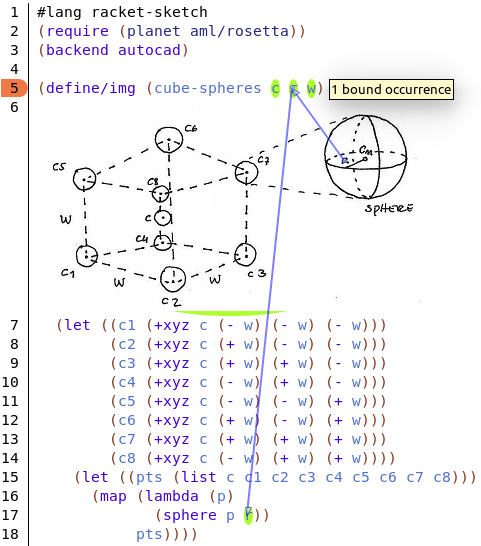
\includegraphics[width=\textwidth]{img/img-code}
                \caption{Searching for ``r'' meaning.}
                \label{fig:img-code1}
        \end{subfigure}%
        ~ %add desired spacing between images, e. g. ~, \quad, \qquad, \hfill etc.
          %(or a blank line to force the subfigure onto a new line)
        \begin{subfigure}{0.5\textwidth}
                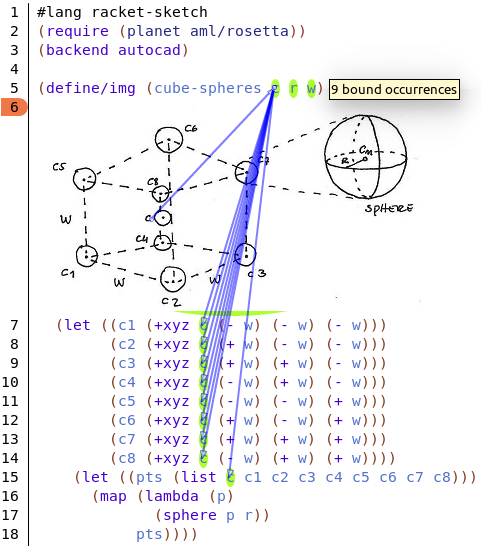
\includegraphics[width=\textwidth]{img/img-code-2}
                \caption{Searching for ``c'' meaning.}
                %\label{}
        \end{subfigure}
        \caption{Contextualizing the code with image.}
        \label{fig:img-code}
\end{figure}

\subsection{DrRacket Properties}

Like DrRacket, our solution initially will target students. The proposed features are supposed to be used for quickly experimenting ideas and to progressively migrate these experiments to a bigger project. However, this interactive environment can be used for either a beginner who wants to understand a piece of code or a professional programmer who needs to test a particular module.

Fortunately, DrRacket is built in the same principle we search for and has some key qualities:

\begin{itemize}
	\item \textbf{Pedagogic.} DrRacket has been a popular environment for introductory courses in programming languages. The environment is designed to guide the student by catching typical mistakes and explain them in terms the students understand. The environment is also useful for professional programmers, due to its sophisticated programming tools, such as the static debugger, and its advanced language features, such as units and mixins.

	\item \textbf{Sophisticated editor.} DrRacket fully integrates a graphics-enriched editor which supports, in addition to plain text, elements such as images, boxes (with comments, Racket code and XML code), etc. DrRacket also displays these elements appropriately in the read-eval-print loop.

	\item \textbf{Extensible.} The main tools of DrRacket environment is implemented using the same \ac{api} that it provides for extension. For example, the debugger, the syntax checker and the stepper, despite of providing different functionalities, these tools implements the same \ac{api}. And this \ac{api} is available for any ordinary tool.
\end{itemize}

However, DrRacket lacks on a mechanism which enables beginner programmers to effortless read the code and also allow them immediately see the result of their actions. In the next section, we present a possible way to integrate these mechanisms in DrRacket.

\subsection{Proposed Architecture}

The Figure~\ref{fig:solution}, presents a publish-subscribe view of the proposed tool. There are two different interactions in this architecture, the first presented by a publish-subscribe and the second by a client-server.

\begin{enumerate}
	\item \texttt{DrRacket UI event manager} acts as an event bus for user-interface events (such as button clicks). Subscription information, i.e. which \ac{ui} events are relevant to our system and which components handle them, is defined at load time when the event manager reads the \textit{plugin} configuration file, the \texttt{info} file. So, when user are working on a editor, an \ac{ui} event is generated and dispatched via implicit invocation to the action handler objects that subscribe to that event.

	\item The manuscripts symbols, present on the image, will be parsed using an \ac{ocr} engine. This engine usually gets an image and returns a text file containing a symbol table with the parsed symbols and its respective coordinates on the image. We expect the \ac{ocr} engine to act as an external service that allows to identify those symbols. For this purpose, in our architecture the \texttt{symbol identifier} component call this service to handle the recognition of symbols in the image.
\end{enumerate}

\begin{figure}[htb]
 \vspace{-15pt}
	\centering
	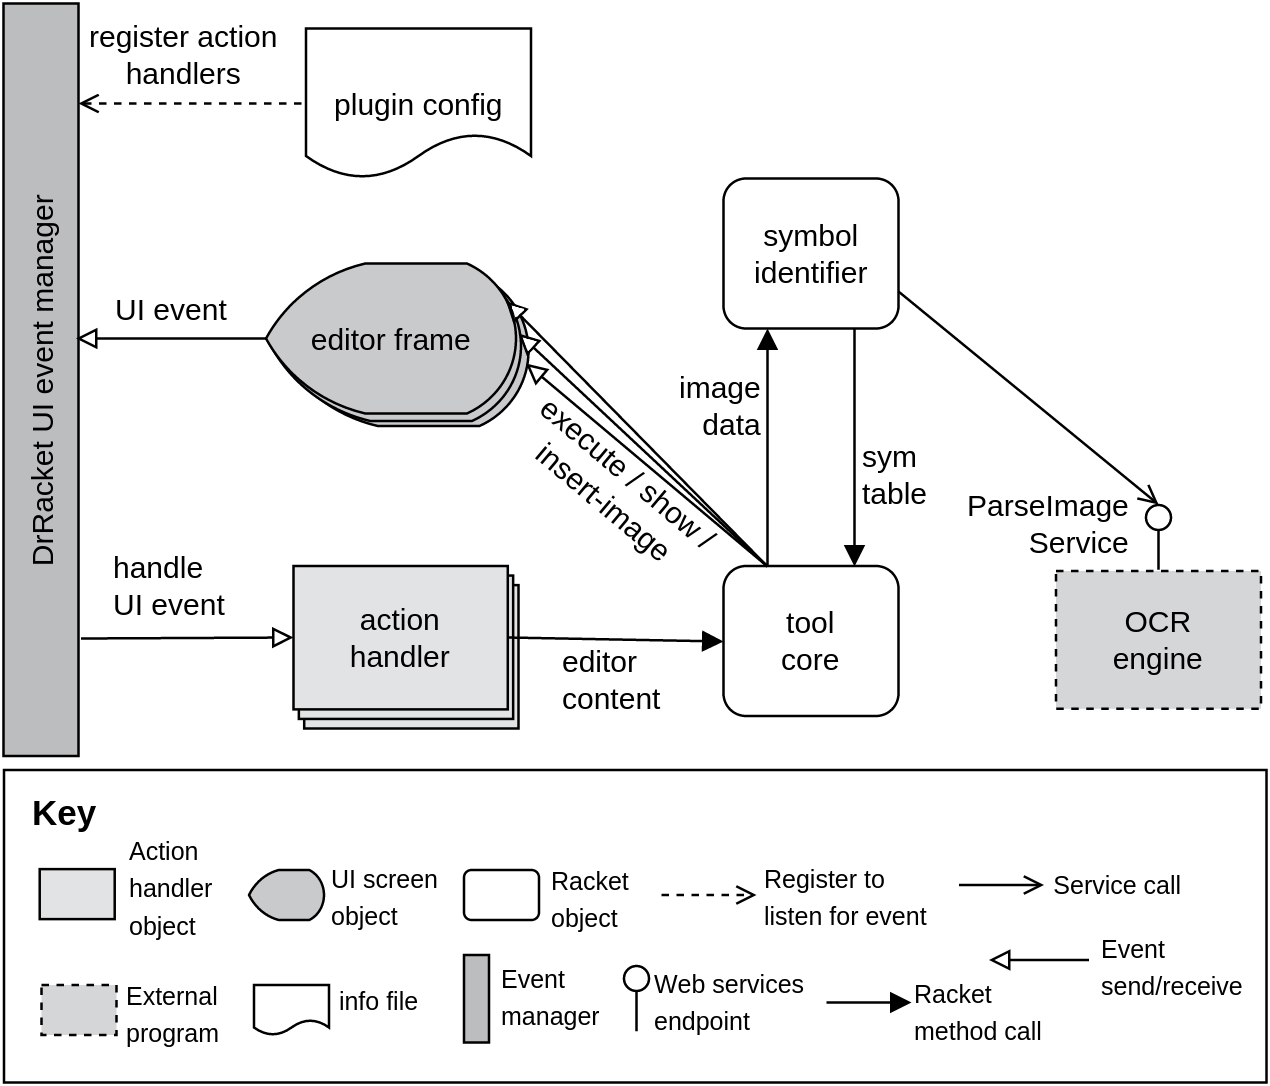
\includegraphics[scale=0.19]{img/solution}
	\vspace{-10pt}
	\caption{Diagram for a publish subscribe view of the proposed architecture.}
	\label{fig:solution}
 \vspace{-10pt}
\end{figure}

The \texttt{tool core} component, in Figure~\ref{fig:solution}, will change the editor based on, mainly, the following events:

\begin{itemize}
	\item \texttt{on-change:} when DrRacket detects that the editor has been modified, it sends the contents of the editor over to action handlers.
	The action handler, in this case is the \texttt{online expansion handler}; a separated place where the code is expanded. \textit{Desired action}: \texttt{execute} the code when the syntax is correct. 

	\item \texttt{on-paint:} this event is sent just before and just after every painting of the editor. Handling this event provide a way to add arbitrary graphics to an editor's display. \textit{Desired action}: \texttt{show} a slider widget when the cursor stops over a literal.

	\item \texttt{on-new-image-snip:} this event is sent when an image is inserted in the editor. The default implementation creates an image snip which is an object with the image information, such as path, format, etc. \textit{Desired action}: get the image and sent it to the \ac{ocr} engine to recognize its symbols and respective coordinates (x, y). Then return an subclass of image snip, adding this extra information.
\end{itemize}

Finally, to connect all pieces of the image recognition we will use a syntactic transformer, i.e. macro. The macro will add a new syntax form into the language grammar, allowing an image to be used as a comment. Very similar to Lisper's comment, we will add a new rule where an image will be between a function declaration and a function body. Basically, the image will be ignored. However, in background, our macro expansion will add to the function body new occurrences of the function parameter. As a result, the DrRacket arrow mechanism will be able to recognize bound occurrences and point to them inside an image.

